\documentclass{article}
\usepackage{graphicx} % Required for inserting images
\usepackage{float}
\usepackage{booktabs}

\title{Final Project EDT}
\author{Santiago Chitiva \\ Valeria Caycedo \\ Samuel Campos \\ Erick Salazar \\ Juan E. Díaz}
\date{May 2026}

\begin{document}

\maketitle

\section{Phase 1: Problem Definition and Data Acquisition}

\subsection{Event Definition and Study Area}

This project revisits the case study analyzed in the Midterm Project: the collapse
of the Kakhovka Dam on June 6, 2023, located on the Dnieper River in Kherson Oblast,
southern Ukraine. The event caused catastrophic downstream flooding and the rapid
drainage of the Kakhovka Reservoir, making it one of the most significant
hydrological disasters in recent European history.

The Region of Interest (ROI) is centered on the area surrounding Nova Kakhovka,
where the effects of reservoir drainage were most clearly observable in satellite
imagery. This ROI was selected based on image availability and the visibility of
hydrological changes in the post-event date (June 18, 2023).

\begin{figure}[H]
    \centering
    \begin{minipage}{0.48\textwidth}
        \centering
        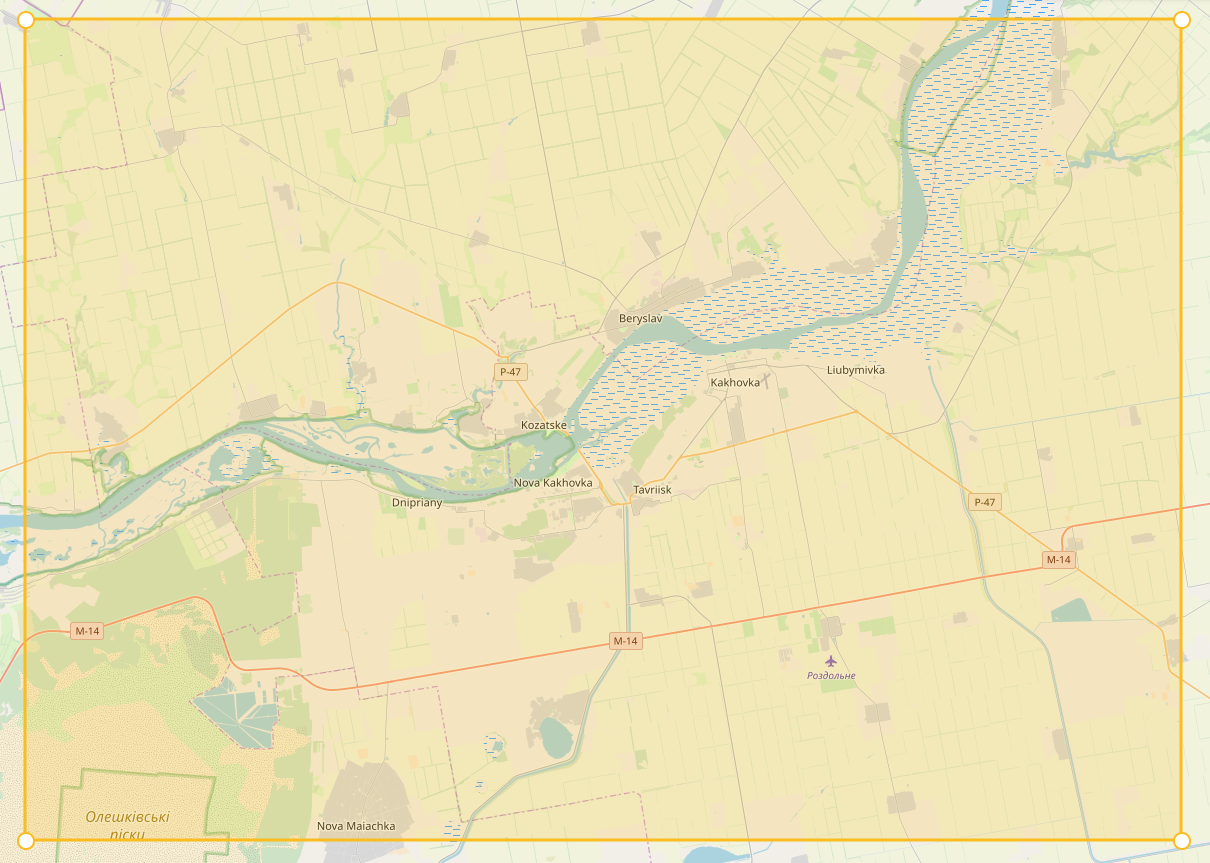
\includegraphics[width=\textwidth]{figures/roi_background_osm.png}
        \caption{ROI on an OpenStreetMap background.}
        \label{fig:roi_osm}
    \end{minipage}
    \hfill
    \begin{minipage}{0.48\textwidth}
        \centering
        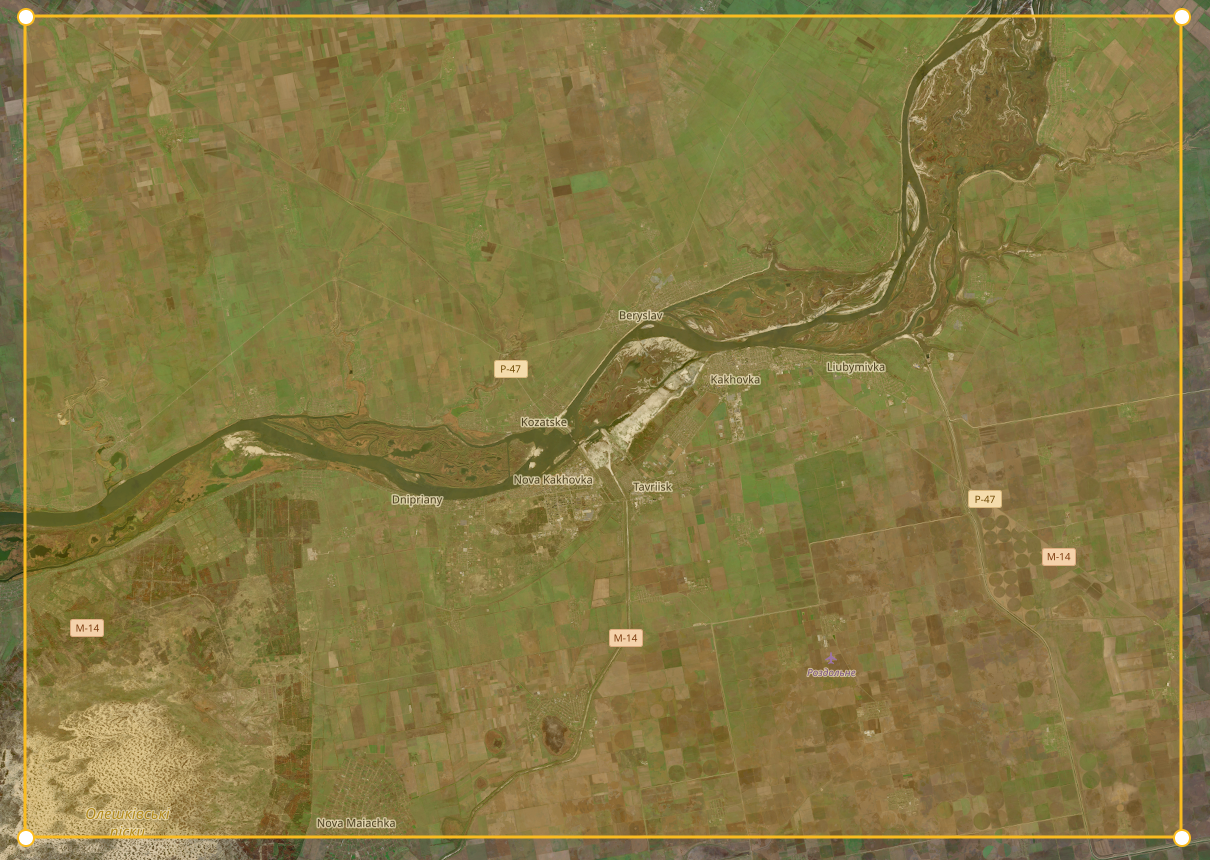
\includegraphics[width=\textwidth]{figures/roi_background_normal.png}
        \caption{ROI on Sentinel-2 image post-event.}
        \label{fig:roi_normal}
    \end{minipage}
\end{figure}

\subsection{Satellite Imagery Metadata}

Two Sentinel-2 Level-2A images were acquired from the Copernicus Open Access Hub.
Table~\ref{tab:imagery_metadata} summarizes their main technical characteristics.

\begin{table}[h]
    \centering
    \caption{Technical characteristics of the satellite imagery used.}
    \label{tab:imagery_metadata}
    \begin{tabular}{lllllll}
        \hline
        \textbf{Date} & \textbf{Satellite} & \textbf{Level} &
        \textbf{Resolution} & \textbf{Cloud Cover} & \textbf{Role} \\
        \hline
        June 18, 2023 & Sentinel-2 A/B & Level-2A & 10 m & $<$30\% & Post-event \\
        \hline
    \end{tabular}
\end{table}

Level-2A products provide Bottom-of-Atmosphere (BOA) reflectance, eliminating the
need for additional atmospheric correction. The bands used for this project span
from the visible to the shortwave infrared spectrum, as detailed in
Table~\ref{tab:bands}.

\begin{table}[h]
    \centering
    \caption{Sentinel-2 spectral bands used for dataset construction.}
    \label{tab:bands}
    \begin{tabular}{cll}
        \hline
        \textbf{Band} & \textbf{Name} & \textbf{Wavelength ($\mu$m)} \\
        \hline
        B2  & Blue                   & 0.490 \\
        B3  & Green                  & 0.560 \\
        B4  & Red                    & 0.665 \\
        B5  & Red Edge 1             & 0.705 \\
        B6  & Red Edge 2             & 0.740 \\
        B7  & Red Edge 3             & 0.783 \\
        B8  & Near-Infrared (NIR)    & 0.842 \\
        B8A & Narrow NIR             & 0.865 \\
        B11 & SWIR 1                 & 1.610 \\
        B12 & SWIR 2                 & 2.190 \\
        \hline
    \end{tabular}
\end{table}

\subsection{Dataset Construction}

To prepare the training dataset for the machine learning phase, pixel values were
extracted from the Sentinel-2 band stack at the locations defined by the training
polygons digitized in QGIS. Each polygon corresponds to one of four land cover
classes: Water, Vegetation, Bare Soil, and Built-up.

\begin{figure}[H]
    \centering
    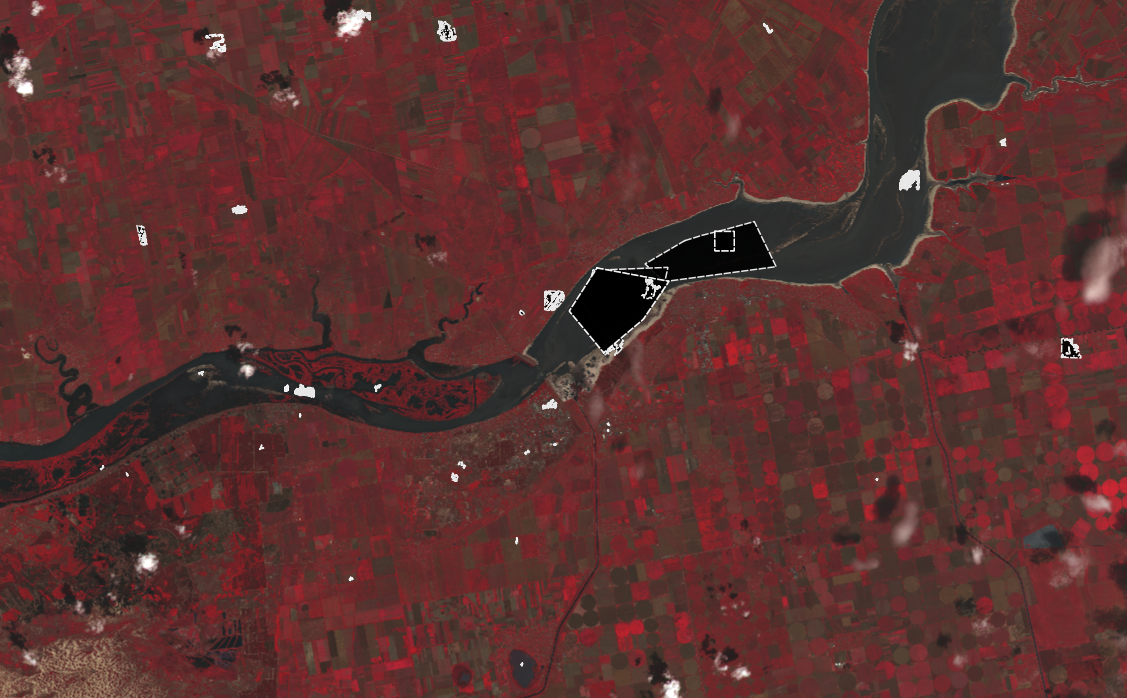
\includegraphics[width=0.85\textwidth]{figures/training_polygons_falsecolor.png}
    \caption{False-color composite (NIR--Red--Green) with digitized training polygons over the post-event study area.}
    \label{fig:training_polygons}
\end{figure}

\begin{figure}[H]
    \centering
    \begin{minipage}{0.48\textwidth}
        \centering
        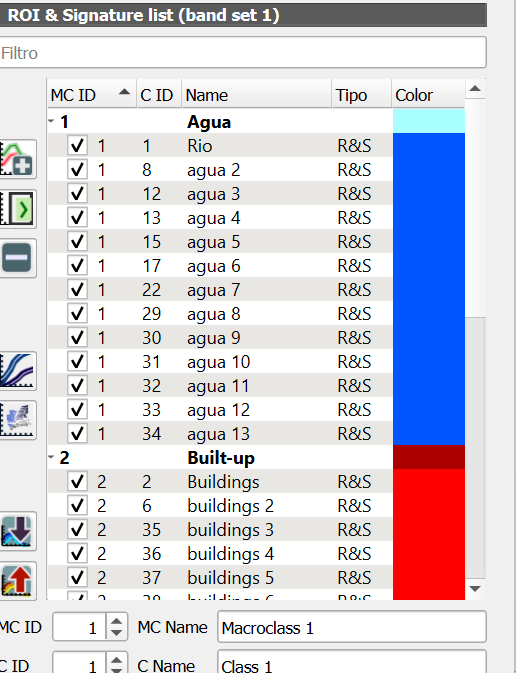
\includegraphics[width=\textwidth]{figures/signature_list_1.png}
        \caption{ROI \& Signature list: clases Water (MC 1) y Built-up (MC 2).}
        \label{fig:sig1}
    \end{minipage}
    \hfill
    \begin{minipage}{0.48\textwidth}
        \centering
        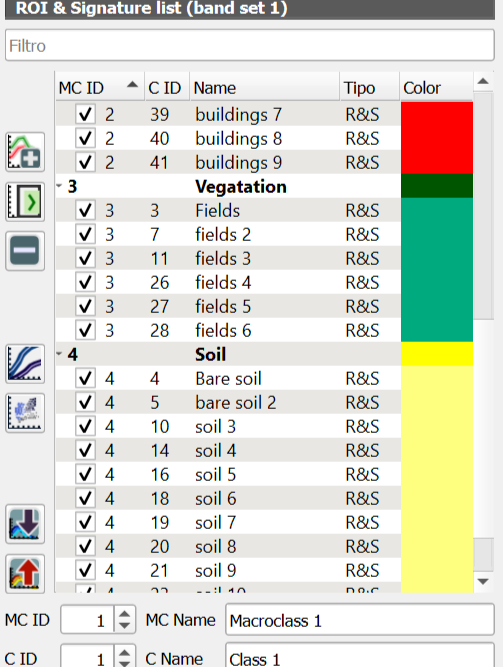
\includegraphics[width=\textwidth]{figures/signature_list_2.png}
        \caption{ROI \& Signature list: clases Vegetation (MC 3) y Soil (MC 4).}
        \label{fig:sig2}
    \end{minipage}
\end{figure}

The extraction was performed using a Python script based on the \texttt{rasterio}
and \texttt{geopandas} libraries. For each pixel falling within a training polygon,
the script records its geographic coordinates (Latitude, Longitude), the reflectance
values for all ten spectral bands, and the corresponding class label. The output was
exported as a Tab-Separated Values (TSV) file, as required for the subsequent
training phase.

Table~\ref{tab:tsv_structure} illustrates the structure of the resulting dataset.

\begin{table}[h]
    \centering
    \caption{Structure of the exported TSV training dataset.}
    \label{tab:tsv_structure}
    \begin{tabular}{lll}
        \hline
        \textbf{Column} & \textbf{Type} & \textbf{Description} \\
        \hline
        Latitude  & Float  & Geographic latitude of the pixel centroid \\
        Longitude & Float  & Geographic longitude of the pixel centroid \\
        B2        & Float  & Blue band reflectance \\
        B3        & Float  & Green band reflectance \\
        B4        & Float  & Red band reflectance \\
        B5        & Float  & Red Edge 1 reflectance \\
        B6        & Float  & Red Edge 2 reflectance \\
        B7        & Float  & Red Edge 3 reflectance \\
        B8        & Float  & NIR band reflectance \\
        B8A       & Float  & Narrow NIR reflectance \\
        B11       & Float  & SWIR 1 reflectance \\
        B12       & Float  & SWIR 2 reflectance \\
        label     & String & Land cover class (Water, Vegetation, Bare Soil, Built-up) \\
        \hline
    \end{tabular}
\end{table}

Table~\ref{tab:dataset_sample} shows the first three extracted pixels for each land cover class.

\begin{table}[H]
    \centering
    \caption{Sample of the training dataset: first three pixels per class (band values in DN).}
    \label{tab:dataset_sample}
    \resizebox{\textwidth}{!}{%
    \begin{tabular}{llccccccccccl}
        \hline
        \textbf{Latitude} & \textbf{Longitude} & \textbf{B2} & \textbf{B3} & \textbf{B4} & \textbf{B5} & \textbf{B6} & \textbf{B7} & \textbf{B8} & \textbf{B8A} & \textbf{B11} & \textbf{B12} & \textbf{Label} \\
        \hline
        46.7608 & 33.3754 & 2194 & 2594 & 2814 & 3081 & 3493 & 3680 & 3706 & 3814 & 3981 & 3641 & Built-up \\
        46.7613 & 33.3728 & 2228 & 2422 & 2636 & 3922 & 4128 & 4250 & 3146 & 4389 & 5874 & 6179 & Built-up \\
        46.7432 & 33.3801 & 3118 & 3508 & 3654 & 3765 & 3625 & 3636 & 3614 & 3530 & 4830 & 5244 & Built-up \\
        \hline
        46.7859 & 33.7286 & 1672 & 2032 & 1980 & 2582 & 3697 & 3947 & 4010 & 4147 & 4130 & 3402 & Soil \\
        46.9410 & 33.3038 & 1637 & 1803 & 2108 & 2274 & 2362 & 2492 & 2582 & 2731 & 4313 & 4164 & Soil \\
        46.9398 & 33.3070 & 1618 & 1822 & 2116 & 2325 & 2395 & 2520 & 2564 & 2732 & 4246 & 4110 & Soil \\
        \hline
        46.8116 & 33.3766 & 1433 & 1647 & 1747 & 2160 & 3027 & 3297 & 3254 & 3573 & 3201 & 2323 & Vegetation \\
        46.8139 & 33.3806 & 1418 & 1698 & 1732 & 2232 & 3184 & 3495 & 3654 & 3789 & 3365 & 2495 & Vegetation \\
        46.8154 & 33.3775 & 1418 & 1693 & 1552 & 2172 & 3293 & 3501 & 3520 & 3749 & 2974 & 2121 & Vegetation \\
        \hline
        46.8072 & 33.4318 & 1930 & 2158 & 2342 & 2509 & 2602 & 2727 & 2814 & 2894 & 2539 & 1949 & Water \\
        46.8025 & 33.4031 & 1750 & 1896 & 1952 & 2074 & 2017 & 2046 & 2130 & 1998 & 1588 & 1474 & Water \\
        46.7926 & 33.4182 & 1693 & 1872 & 2082 & 2246 & 2365 & 2422 & 2532 & 2712 & 4124 & 2849 & Water \\
        \hline
    \end{tabular}}
\end{table}

\section{Phase 2: Pre-processing and Training}

\subsection{Pre-processing}

Before training the machine learning models, several pre-processing operations were applied to the dataset in order to improve data consistency, ensure
fair model evaluation, and optimize classification performance.

The exported TSV dataset contained spectral reflectance values extracted from Sentinel-2 imagery for four land cover classes: Built-up, Soil, Vegetation,
and Water. Each sample represented a single pixel and included ten spectral features corresponding to bands B2, B3, B4, B5, B6, B7, B8, B8A, B11, and B12.

The initial extraction yielded a highly imbalanced dataset of 547{,}173 pixels,
with a severe class disparity as shown in Table~\ref{tab:raw_distribution}.

\begin{table}[H]
    \centering
    \caption{Raw pixel distribution before balancing.}
    \label{tab:raw_distribution}
    \begin{tabular}{lc}
        \hline
        \textbf{Class} & \textbf{Pixel count} \\
        \hline
        Water      & 510{,}071 \\
        Soil       & 22{,}171 \\
        Vegetation & 13{,}379 \\
        Built-up   & 1{,}552 \\
        \hline
        \textbf{Total} & 547{,}173 \\
        \hline
    \end{tabular}
\end{table}

Water dominated the dataset with over 93\% of all pixels, which would have
caused severe bias toward that class in any trained model. To correct this,
additional training polygons were digitized specifically for the Built-up class,
and the dataset was subsequently balanced by random undersampling to 2{,}027
pixels per class, yielding a final balanced dataset of 8{,}108 samples evenly
distributed among the four categories.

Prior to model training, the dataset was inspected for missing or invalid values. Since the spectral extraction process was performed directly from
Sentinel-2 Level-2A products, no significant missing data were detected and no additional interpolation procedures were required.

The categorical class labels were encoded into numerical representations in order to be compatible with the machine learning algorithms. Subsequently, the
dataset was divided into training and testing subsets using stratified sampling to preserve the original class distribution. Approximately 70\% of the
samples were used for training and 30\% for testing.

Feature scaling was also applied during the pre-processing stage. Since some algorithms, particularly Artificial Neural Networks (ANN) and K-Nearest
Neighbors (KNN), are sensitive to differences in feature magnitude, the spectral bands were normalized using standard scaling. This transformation ensured
that all features contributed proportionally during the optimization process.

For the ANN implementation, the target labels were additionally transformed into categorical representations suitable for multiclass classification with a
softmax output layer. Regularization techniques such as Dropout were later used during training to reduce the risk of overfitting.

Overall, the pre-processing stage ensured that the spectral dataset was properly formatted, balanced, normalized, and ready for supervised land cover
classification using the selected machine learning approaches.

\subsection{Models}

\subsubsection{Decision Trees (DT)}
The following table summarizes the hyperparameter configurations tested during the model optimization process.

\begin{table}[H]
    \centering
    \caption{Hyperparameter search space for the Decision Tree classifier.}
    \label{tab:dt_hpo}
    \begin{tabular}{ll}
        \hline
        \textbf{Hyperparameter} & \textbf{Values tested} \\
        \hline
        \texttt{criterion}         & gini, entropy, log\_loss \\
        \texttt{max\_depth}        & None, 5, 10, 15, 20 \\
        \texttt{min\_samples\_split} & 2, 5, 10 \\
        \texttt{min\_samples\_leaf}  & 1, 2, 4 \\
        \hline
        \multicolumn{2}{l}{\textit{Method: 5-fold StratifiedKFold, scoring: F1-macro}} \\
        \hline
    \end{tabular}
\end{table}

The results show excellent performance of the Decision Tree model in the post-event classification problem. An overall accuracy of $98.56\%$ means that, out of 2433 test samples, almost all were correctly classified. Furthermore, a Kappa coefficient of $0.9808$ indicates very high agreement beyond chance, confirming that the model is actually learning useful spectral patterns rather than simply exploiting the class distribution.

\begin{table}[H]
\centering
\caption{Classification Report for the Decision Tree Model}
\label{tab:classification_report}
\begin{tabular}{lcccc}
\hline
\textbf{Class} & \textbf{Precision} & \textbf{Recall} & \textbf{F1-score} & \textbf{Support} \\
\hline
Built-up   & 0.9806 & 0.9951 & 0.9878 & 608 \\
Soil       & 0.9867 & 0.9737 & 0.9801 & 608 \\
Vegetation & 0.9870 & 0.9984 & 0.9927 & 609 \\
Water      & 0.9883 & 0.9753 & 0.9818 & 608 \\
\hline

\end{tabular}
\end{table}

The macro F1-score of $0.9856$ reinforces this conclusion because it averages performance across classes while giving equal importance to each one, and it still remains very high. Likewise, the weighted F1-score of $0.9856$ closely matches the macro value, suggesting balanced performance and the absence of clearly disadvantaged classes. In other words, the model not only performs well globally, but also consistently across all land-cover categories.

\begin{figure}[H]
    \centering
    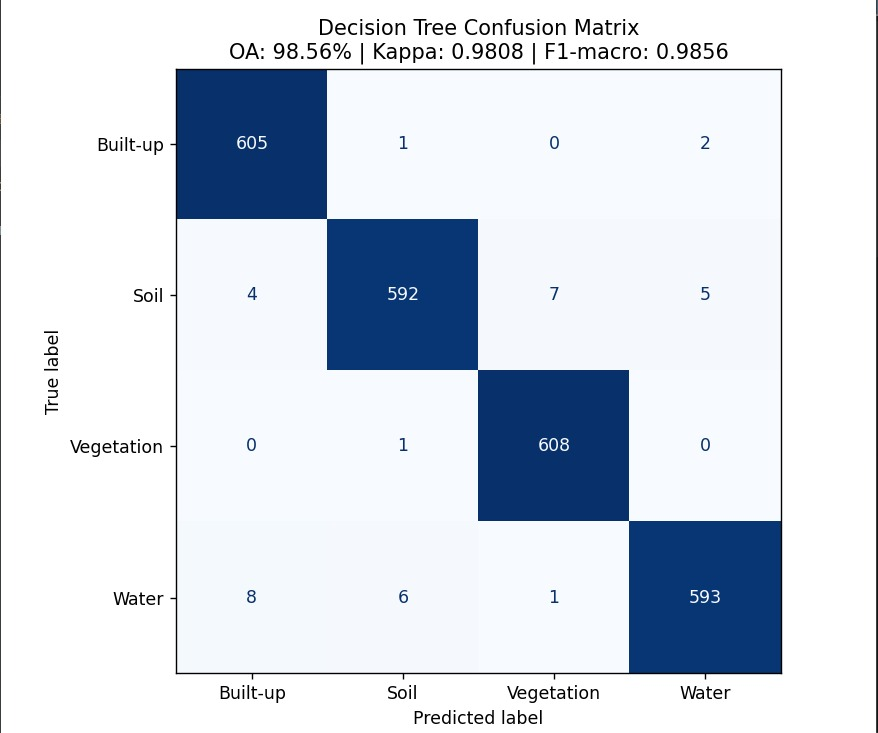
\includegraphics[width=0.5\linewidth]{figures/DT_confusion_matrix.png}
    \caption{Confusion matrix obtained from the Decision Trees.}
    \label{fig:placeholder}
\end{figure}

The confusion matrix shows that \textit{Vegetation} is the strongest class ($608/609$ correctly classified samples), followed by \textit{Built-up} ($605/608$). The most frequent confusions occur between \textit{Soil} and \textit{Water}, and to a lesser extent between \textit{Water} and \textit{Built-up}. This behavior is expected in satellite imagery because of local spectral similarities, mixed pixels, and humidity or shadow effects. Even with these specific confusions, the number of errors is very small compared to the total number of samples and does not compromise the overall quality of the model.

Finally, it can be concluded that the Decision Tree model provides a good performance for the Kakhovka scene and achieves effective land-cover separation.

\subsubsection{Support Vector Machine (SVM)}

A Support Vector Machine (SVM) classifier was implemented to perform supervised land cover classification using the spectral information extracted from
the Sentinel-2 imagery. SVM is a widely used machine learning algorithm in remote sensing applications due to its strong performance in high-dimensional
datasets and its ability to separate classes using optimal decision boundaries.

The training dataset, evenly distributed among the four land cover classes: Built-up, Soil, Vegetation, and Water. Each
sample corresponds to a single pixel and contains the reflectance values from the ten spectral bands used in this project.

Before training, the dataset was divided into training and testing subsets using a stratified split in order to preserve the class distribution.
Approximately 70\% of the samples were used for training and 30\% for evaluation.

\begin{table}[H]
    \centering
    \caption{Hyperparameter search space for the SVM classifier.}
    \label{tab:svm_hpo}
    \begin{tabular}{ll}
        \hline
        \textbf{Hyperparameter} & \textbf{Values tested} \\
        \hline
        \texttt{kernel}  & RBF (fixed) \\
        \texttt{C}       & 0.5, 1.0, 1.5, \ldots, 15.0 (step 0.5, 30 values) \\
        \texttt{gamma}   & scale (fixed) \\
        \hline
        \multicolumn{2}{l}{\textit{Method: sequential evaluation on test set}} \\
        \hline
    \end{tabular}
\end{table}

The SVM model achieved an Overall Accuracy of 99.75\%, demonstrating excellent classification performance across all land cover categories. Precision,
recall, and F1-score values were close to 1.00 for every class, indicating that the spectral signatures extracted from the Sentinel-2 bands provide strong
class separability.

Table~\ref{tab:svm_results} summarizes the evaluation metrics obtained during testing.

\begin{table}[h]
  \centering
  \caption{Classification report for the SVM model.}
  \label{tab:svm_results}
  \begin{tabular}{lcccc}
    \hline
    \textbf{Class} & \textbf{Precision} & \textbf{Recall} & \textbf{F1-score} & \textbf{Support} \\
    \hline
    Built-up   & 1.00 & 1.00 & 1.00 & 608 \\
    Soil       & 1.00 & 0.99 & 1.00 & 608 \\
    Vegetation & 0.99 & 1.00 & 1.00 & 609 \\
    Water      & 1.00 & 1.00 & 1.00 & 608 \\
    \hline
  \end{tabular}
\end{table}

The confusion matrix shown in Figure~\ref{fig:svm_cm} confirms the high classification accuracy of the model. Most samples were correctly classified, with
only a very small number of misclassifications between spectrally similar classes.

\begin{figure}[H]
  \centering
  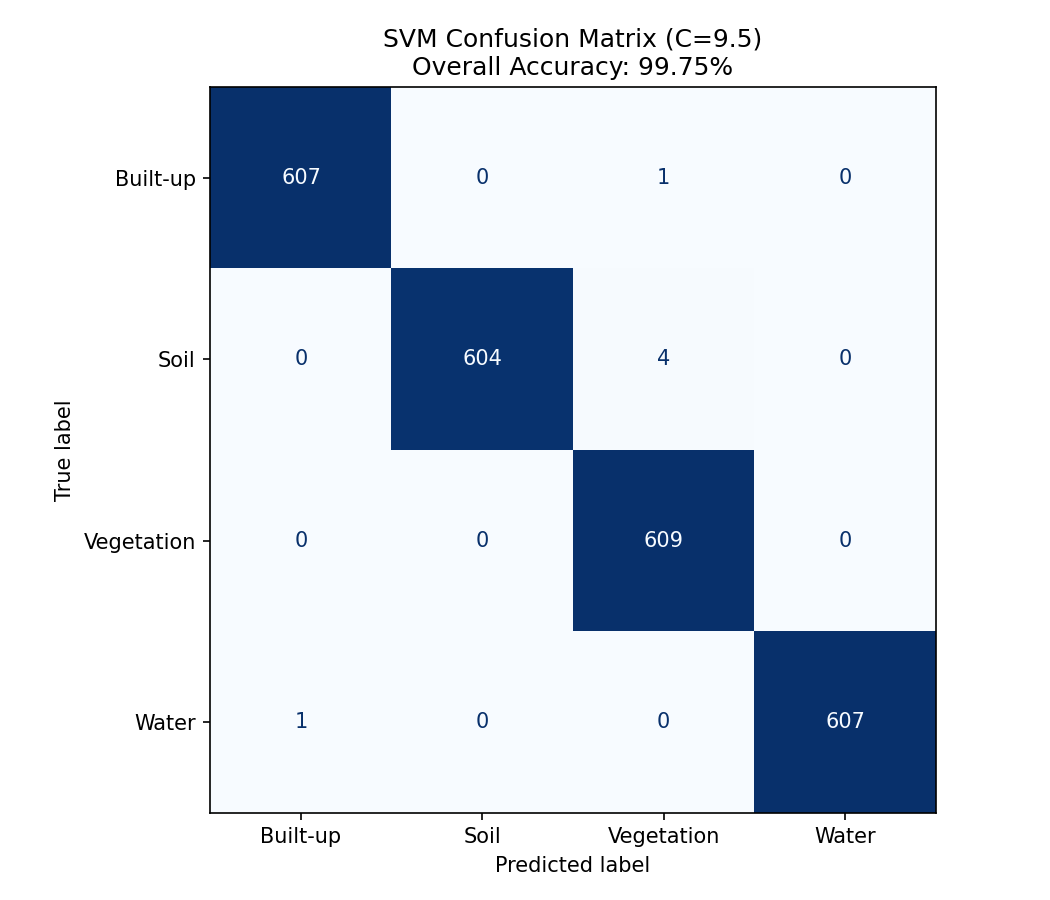
\includegraphics[width=0.75\linewidth]{figures/svm_confusion_matrix.png}
  \caption{Confusion matrix obtained from the SVM classifier.}
  \label{fig:svm_cm}
\end{figure}

These results indicate that the SVM model is highly effective for multispectral land cover classification using Sentinel-2 imagery and provides a strong
baseline for comparison with the other machine learning approaches evaluated in this project.

\subsubsection{Artificial Neural Networks (ANN)}

An Artificial Neural Network (ANN) model was implemented to evaluate the performance of deep learning techniques for multispectral land cover
classification. Neural networks are capable of learning complex nonlinear relationships between spectral features and target classes, making them highly
suitable for remote sensing applications involving high-dimensional data.

The ANN was trained using the same dataset employed for the SVM classifier, containing 8108 labeled pixel samples equally distributed among the classes
Built-up, Soil, Vegetation, and Water. Each sample contains the reflectance values corresponding to the ten Sentinel-2 spectral bands selected for this
study.

Prior to training, the dataset was normalized and divided into training and testing subsets using a stratified split. Approximately 70\% of the data was
used for training, while the remaining 30\% was reserved for model evaluation.

The neural network architecture consisted of multiple fully connected dense layers with ReLU activation functions and Dropout regularization layers to
reduce overfitting. The final output layer used a softmax activation function to perform multiclass classification across the four land cover categories.

\begin{table}[H]
    \centering
    \caption{Hyperparameter search space for the ANN classifier.}
    \label{tab:ann_hpo}
    \begin{tabular}{ll}
        \hline
        \textbf{Hyperparameter} & \textbf{Values tested} \\
        \hline
        \texttt{learning\_rate} & 0.1, 0.05, 0.01, 0.005, 0.001, 0.0005, 0.0001 \\
        \texttt{optimizer}      & Adam (fixed) \\
        \texttt{epochs}         & 50 (fixed) \\
        \texttt{batch\_size}    & 32 (fixed) \\
        \texttt{dropout}        & 0.3 (fixed) \\
        \texttt{architecture}   & Dense(64)--Dropout--Dense(128)--Dropout--Dense(64)--Softmax \\
        \hline
        \multicolumn{2}{l}{\textit{Method: sequential evaluation on test set}} \\
        \hline
    \end{tabular}
\end{table}

The model was trained for 50 epochs and achieved a final Overall Accuracy of 99.59\% on the testing dataset. The training history demonstrated stable
convergence and high validation accuracy throughout the training process.

Table~\ref{tab:ann_results} summarizes the classification metrics obtained for the ANN model.

\begin{table}[h]
    \centering
    \caption{Classification report for the ANN model.}
    \label{tab:ann_results}
    \begin{tabular}{lcccc}
        \hline
        \textbf{Class} & \textbf{Precision} & \textbf{Recall} & \textbf{F1-score} & \textbf{Support} \\
        \hline
        Built-up   & 1.00 & 1.00 & 1.00 & 608 \\
        Soil       & 0.99 & 1.00 & 0.99 & 608 \\
        Vegetation & 1.00 & 1.00 & 1.00 & 609 \\
        Water      & 1.00 & 0.99 & 1.00 & 608 \\
        \hline
    \end{tabular}
\end{table}

Figure~\ref{fig:ann_cm} presents the confusion matrix generated from the ANN predictions. The matrix indicates that the vast majority of samples were
correctly classified, with only minimal confusion between a few spectrally similar classes.

\begin{figure}[H]
    \centering
    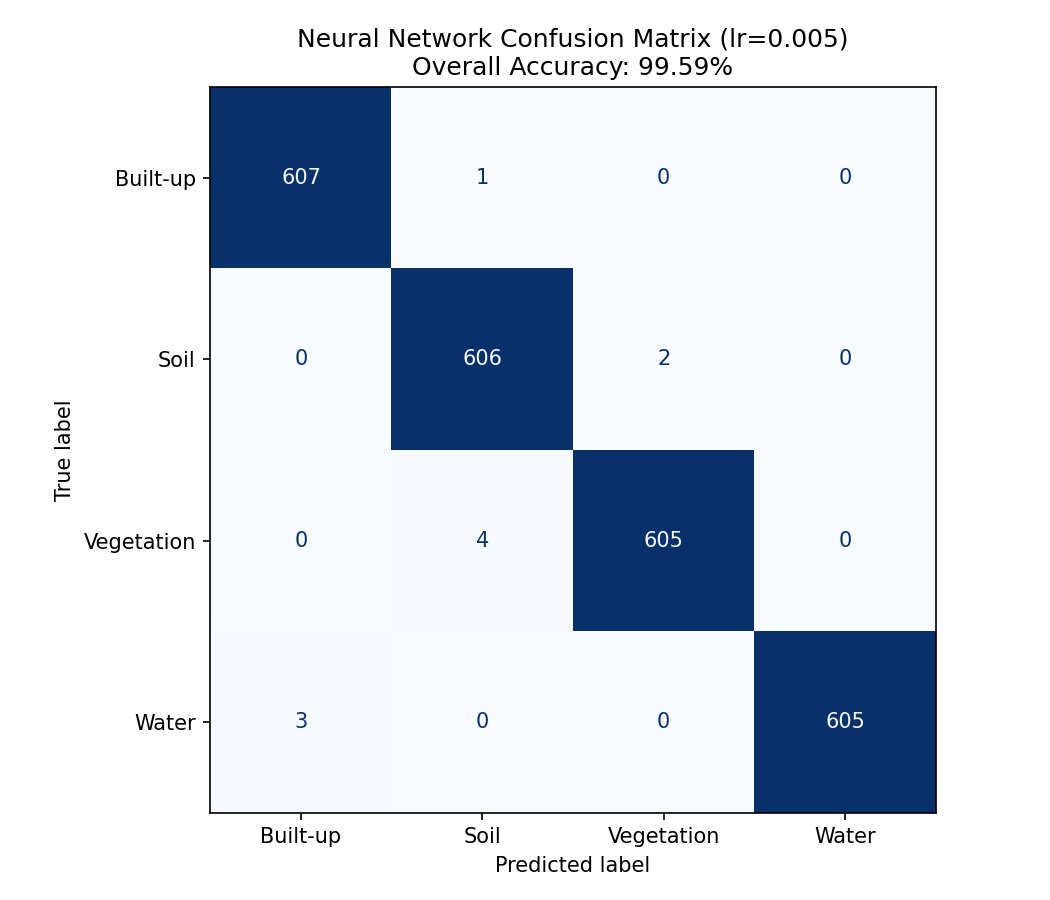
\includegraphics[width=0.75\linewidth]{figures/nn_confusion_matrix.png}
    \caption{Confusion matrix obtained from the ANN classifier.}
    \label{fig:ann_cm}
\end{figure}

Figure~\ref{fig:ann_history} shows the training history of the neural network, including the evolution of training and validation accuracy during the
learning process. The results demonstrate rapid convergence and stable generalization performance.

\begin{figure}[H]
    \centering
    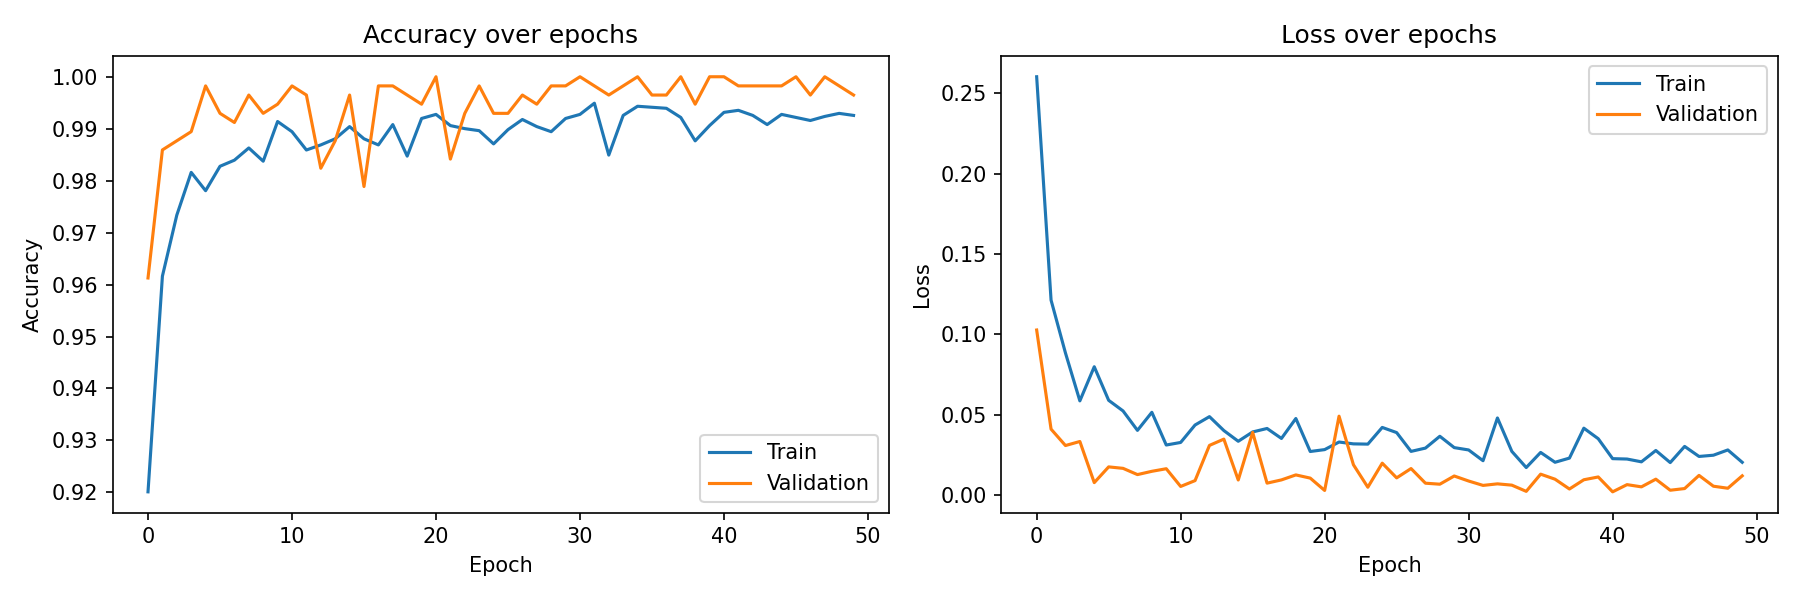
\includegraphics[width=0.85\linewidth]{figures/nn_training_history.png}
    \caption{Training and validation accuracy history for the ANN model.}
    \label{fig:ann_history}
\end{figure}

The ANN model achieved performance comparable to the SVM classifier, confirming that deep learning approaches can effectively model the spectral behavior
of different land cover types using Sentinel-2 multispectral imagery.

\subsubsection{K-Nearest Neighbor (KNN)}
The KNN classifier was trained using an 80/20 train-test split with stratification
across all four land cover classes. Prior to training, all spectral band values were
normalized using standard scaling, as KNN relies on Euclidean distance and is sensitive
to differences in feature magnitude. Hyperparameter optimization was performed via
5-fold cross-validation over a grid of candidate values for the number of neighbors,
weighting scheme, and distance metric.

\begin{table}[H]
    \centering
    \caption{Hyperparameter search space for the KNN classifier.}
    \label{tab:knn_hpo}
    \begin{tabular}{ll}
        \hline
        \textbf{Hyperparameter} & \textbf{Values tested} \\
        \hline
        \texttt{n\_neighbors} & 3, 5, 7, 9, 11 \\
        \texttt{weights}      & uniform, distance \\
        \texttt{metric}       & Euclidean (fixed) \\
        \hline
        \multicolumn{2}{l}{\textit{Method: 5-fold GridSearchCV, scoring: F1-macro}} \\
        \hline
    \end{tabular}
\end{table}

The optimal configuration found was $K = 3$, uniform weighting, and Euclidean distance,
achieving a macro-averaged F1-Score of 0.9943 during cross-validation. Table~\ref{tab:knn_metrics}
summarizes the per-class performance metrics obtained on the test set, and
Table~\ref{tab:knn_cm} presents the corresponding confusion matrix.

\begin{table}[H]
    \centering
    \caption{Per-class performance metrics for the KNN classifier.}
    \label{tab:knn_metrics}
    \begin{tabular}{lcccc}
        \hline
        \textbf{Class} & \textbf{Precision} & \textbf{Recall} & \textbf{F1-Score} & \textbf{Support} \\
        \hline
        Built-up   & 0.9975 & 0.9951 & 0.9963 & 406 \\
        Soil       & 0.9975 & 0.9926 & 0.9950 & 405 \\
        Vegetation & 0.9927 & 1.0000 & 0.9963 & 406 \\
        Water      & 0.9975 & 0.9975 & 0.9975 & 405 \\
        \hline
        \textbf{Overall Accuracy} & \multicolumn{4}{c}{99.63\%} \\
        \textbf{Kappa Coefficient} & \multicolumn{4}{c}{0.9951} \\
        \hline
    \end{tabular}
\end{table}

\begin{table}[H]
    \centering
    \caption{Confusion matrix for the KNN classifier (rows = predicted, columns = reference).}
    \label{tab:knn_cm}
    \begin{tabular}{lcccc}
        \hline
        & \textbf{Built-up} & \textbf{Soil} & \textbf{Vegetation} & \textbf{Water} \\
        \hline
        \textbf{Built-up}   & 404 & 1 & 1 & 0 \\
        \textbf{Soil}       & 0 & 402 & 2 & 1 \\
        \textbf{Vegetation} & 0 & 0 & 406 & 0 \\
        \textbf{Water}      & 1 & 0 & 0 & 404 \\
        \hline
    \end{tabular}
\end{table}

\begin{figure}[H]
    \centering
    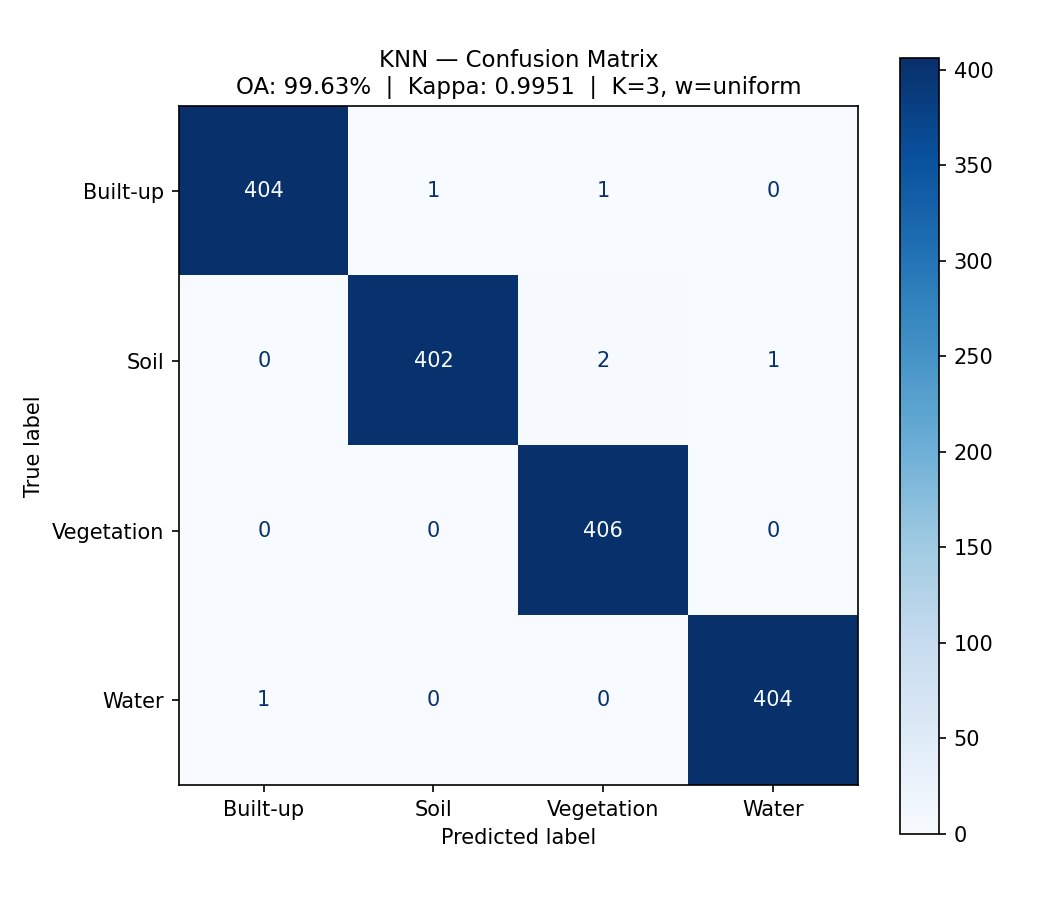
\includegraphics[width=0.75\textwidth]{figures/knn_confusion_matrix.png}
    \caption{Confusion matrix for the KNN classifier ($K=3$, uniform weights,
    Euclidean distance). OA = 99.63\%, Kappa = 0.9951.}
    \label{fig:knn_cm}
\end{figure}

\subsubsection{Naive Bayes (NB)}
The fifth supervised learning architecture implemented in this project was the Naive Bayes classifier. This model is based on Bayes' theorem and estimates the probability that a pixel belongs to a given land-cover class according to its spectral response. In this case, the input variables correspond to the Sentinel-2 spectral bands extracted during the dataset construction stage.

Since the spectral bands are continuous numerical variables, the selected implementation was Gaussian Naive Bayes. This variant assumes that the values of each feature follow a Gaussian distribution within each class. Although the model assumes conditional independence between the spectral bands, which is a strong simplification for multispectral satellite data, it provides a useful probabilistic baseline for comparison against more complex models such as Decision Trees, Support Vector Machines, Artificial Neural Networks, and K-Nearest Neighbors.

The model was trained using the tabular dataset generated from the training polygons. The input features were the spectral bands B2, B3, B4, B5, B6, B7, B8, B8A, B11, and B12, while the target variable was the land-cover class label. The dataset was divided into training and testing subsets, preserving the class distribution. The final split contained 5675 training samples and 2433 testing samples.

A hyperparameter search was performed over the \texttt{var\_smoothing} parameter. The best value obtained was:

\begin{equation}
\texttt{var\_smoothing} = 1 \times 10^{-12}
\end{equation}

This value was used to train the final Gaussian Naive Bayes model.

\begin{table}[H]
\centering
\caption{Summary metrics for the Gaussian Naive Bayes classifier.}
\label{tab:nb_summary_metrics}
\begin{tabular}{lc}
\toprule
\textbf{Metric} & \textbf{Value} \\
\midrule
Best \texttt{var\_smoothing} & $1.0 \times 10^{-12}$ \\
Cross-validation F1 macro & 0.8518 \\
Overall accuracy & 0.8442 \\
Kappa coefficient & 0.7923 \\
F1 macro & 0.8444 \\
F1 weighted & 0.8445 \\
Training samples & 5675 \\
Testing samples & 2433 \\
\bottomrule
\end{tabular}
\end{table}

The obtained overall accuracy was 0.8442, meaning that approximately 84.42\% of the test pixels were correctly classified. The Kappa coefficient reached 0.7923, indicating a strong level of agreement between the predicted and reference classes beyond random chance. The F1 macro score was 0.8444, showing that the classifier achieved balanced performance across the four land-cover categories.

\begin{figure}[H]
\centering
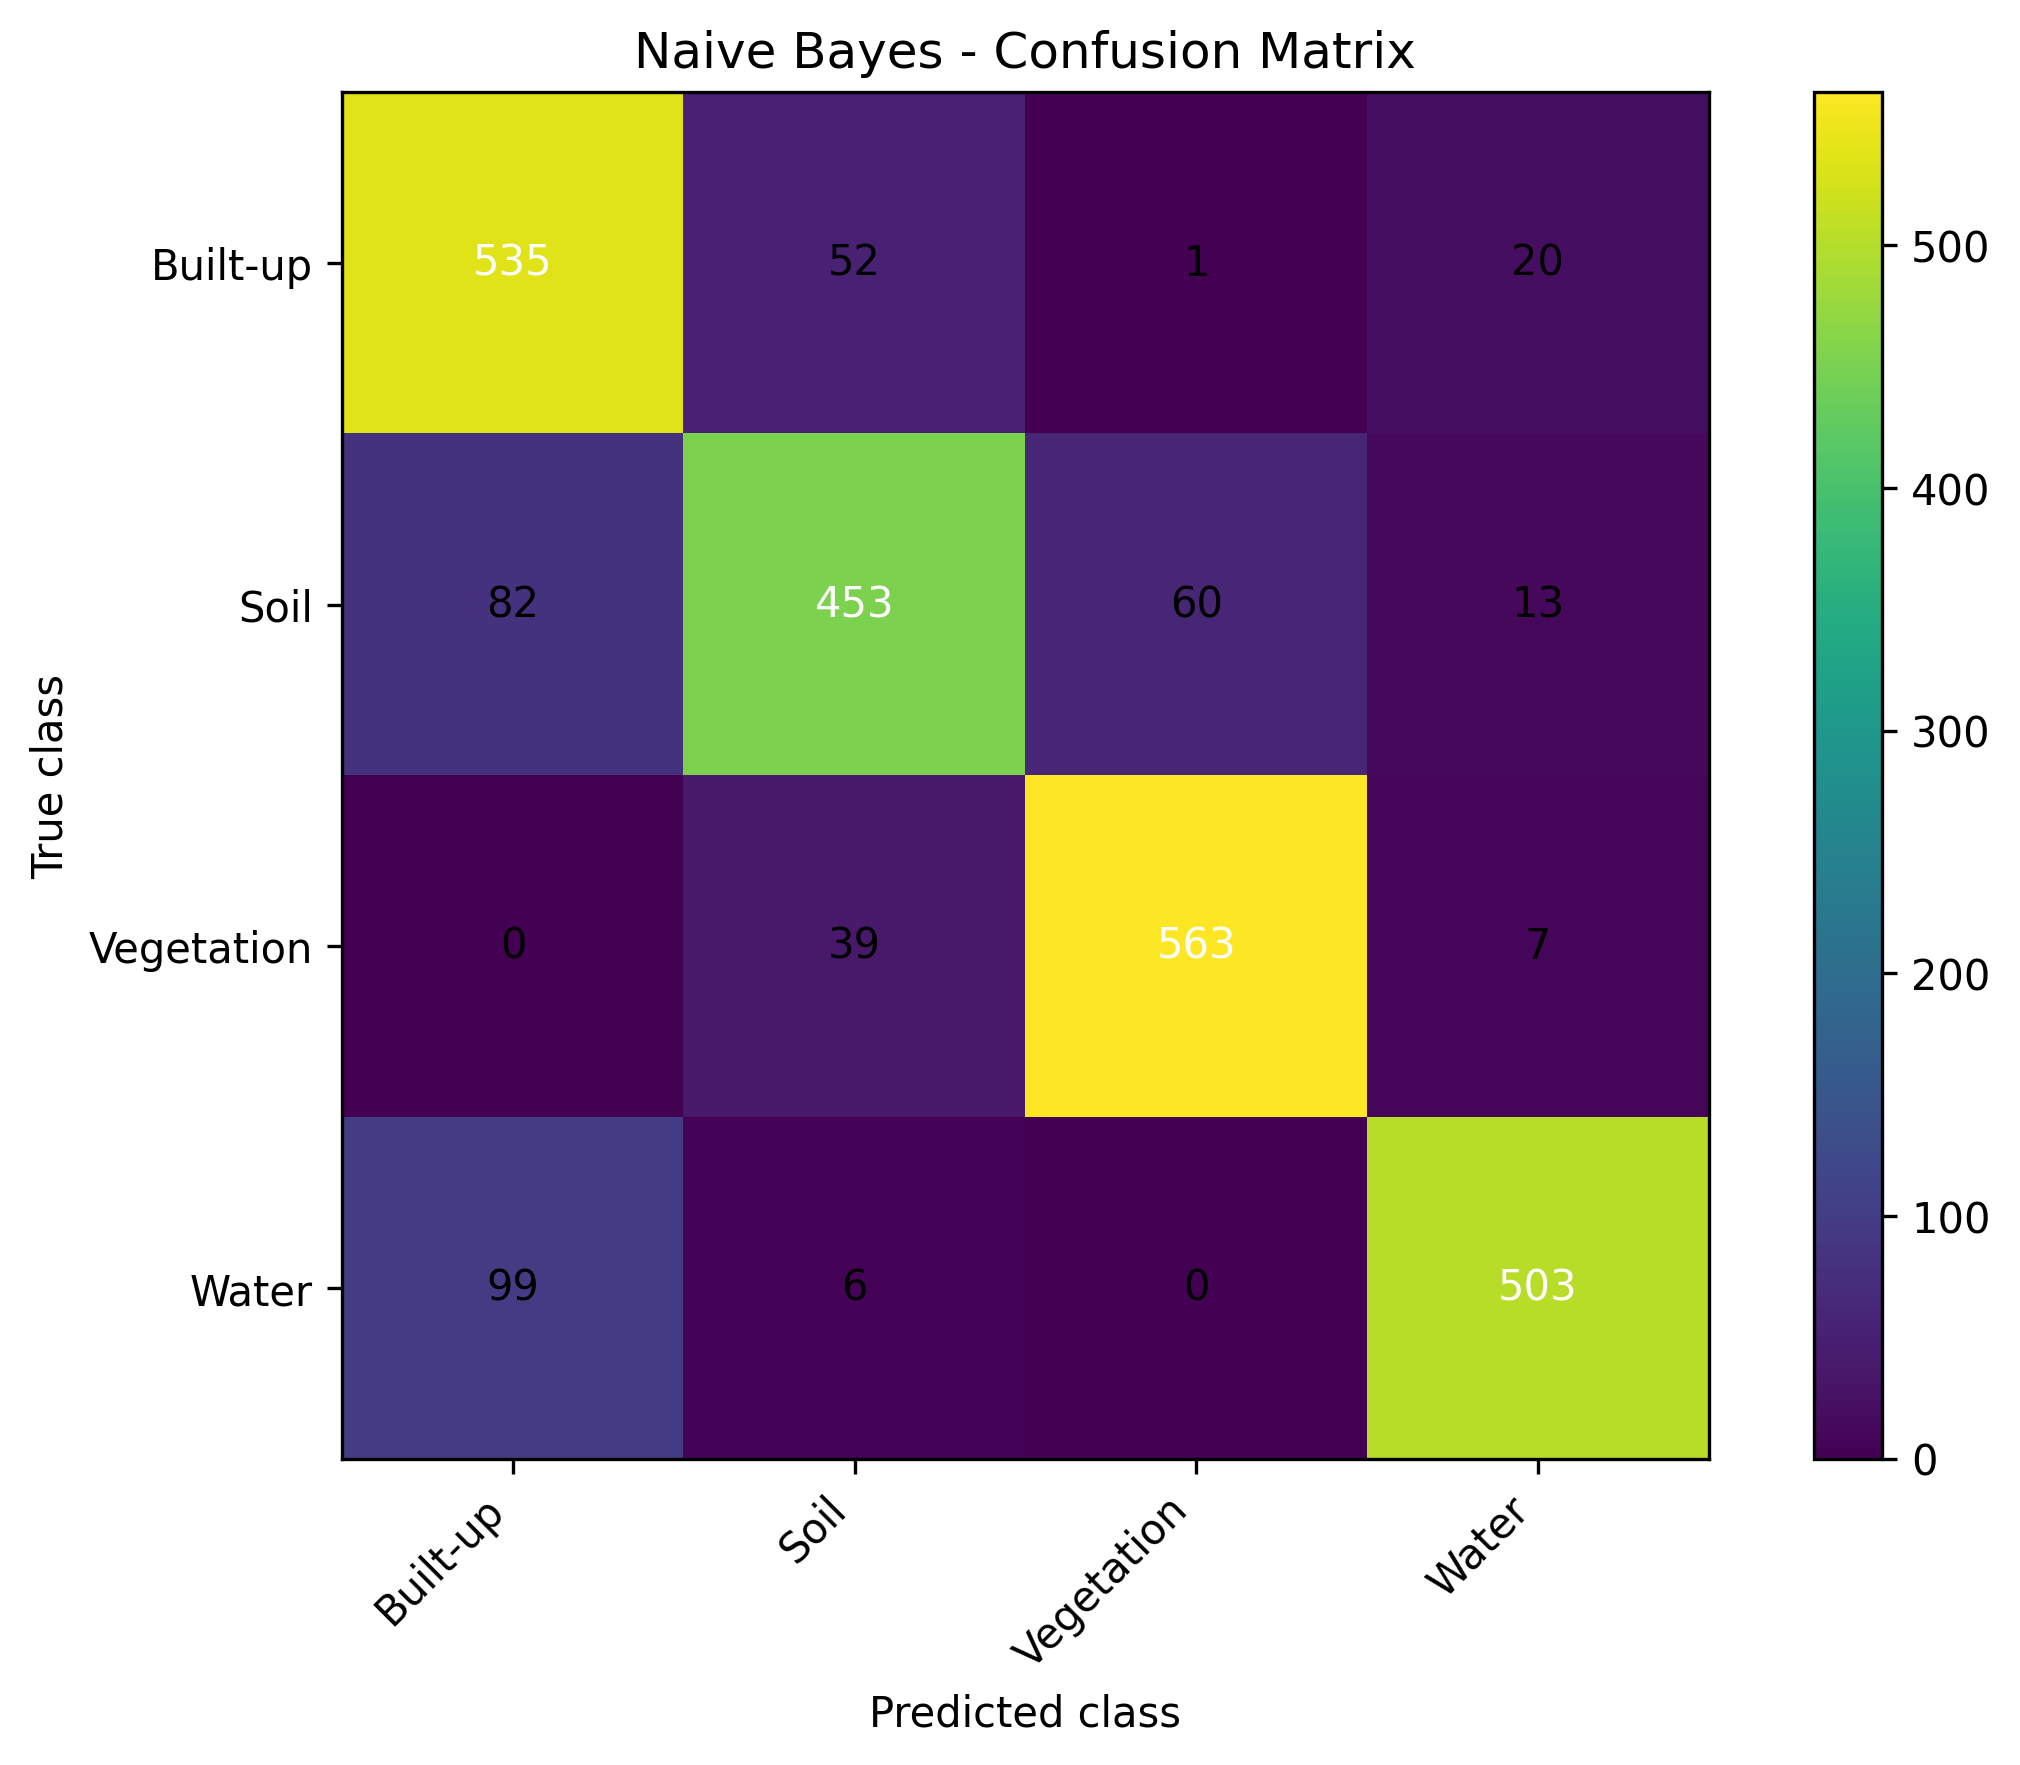
\includegraphics[width=0.85\textwidth]{figures/nb_confusion_matrix.png}
\caption{Confusion matrix obtained with the Gaussian Naive Bayes classifier.}
\label{fig:nb_confusion_matrix}
\end{figure}

\begin{table}[H]
\centering
\caption{Confusion matrix for the Gaussian Naive Bayes classifier.}
\label{tab:nb_confusion_matrix}
\begin{tabular}{lcccc}
\toprule
\textbf{True / Predicted} & \textbf{Built-up} & \textbf{Soil} & \textbf{Vegetation} & \textbf{Water} \\
\midrule
Built-up    & 535 & 52  & 1   & 20 \\
Soil        & 82  & 453 & 60  & 13 \\
Vegetation  & 0   & 39  & 563 & 7  \\
Water       & 99  & 6   & 0   & 503 \\
\bottomrule
\end{tabular}
\end{table}

The confusion matrix shows that the model performed well for all classes, with the highest number of correct predictions located along the main diagonal. Vegetation was the best classified class, with 563 correctly predicted pixels and an F1-score of 0.9132. This indicates that vegetation has a clearly distinguishable spectral signature in the selected Sentinel-2 bands.

Water also obtained strong results, with 503 correctly classified pixels and an F1-score of 0.8740. However, 99 water pixels were incorrectly classified as built-up areas. This confusion may be associated with spectral similarities in dark or low-reflectance regions, shadows, or mixed pixels near the boundaries between flooded and urbanized zones.

Built-up areas achieved 535 correct predictions and an F1-score of 0.8082. The main confusion for this class occurred with soil, where 52 built-up pixels were classified as soil. This behavior is expected in post-event satellite imagery, since exposed surfaces, debris, dry soil, and artificial materials may present similar spectral responses.

The soil class obtained the lowest F1-score among the four classes, with a value of 0.7824. The main errors occurred between soil and built-up areas, with 82 soil pixels classified as built-up, and between soil and vegetation, with 60 soil pixels classified as vegetation. This suggests that soil is the most spectrally ambiguous class in the current dataset.

\begin{table}[H]
\centering
\caption{Classification report for the Gaussian Naive Bayes classifier.}
\label{tab:nb_classification_report}
\begin{tabular}{lcccc}
\toprule
\textbf{Class} & \textbf{Precision} & \textbf{Recall} & \textbf{F1-score} & \textbf{Support} \\
\midrule
Built-up   & 0.7472 & 0.8799 & 0.8082 & 608 \\
Soil       & 0.8236 & 0.7451 & 0.7824 & 608 \\
Vegetation & 0.9022 & 0.9245 & 0.9132 & 609 \\
Water      & 0.9263 & 0.8273 & 0.8740 & 608 \\
\midrule
Macro avg.    & 0.8499 & 0.8442 & 0.8444 & 2433 \\
Weighted avg. & 0.8499 & 0.8442 & 0.8445 & 2433 \\
\bottomrule
\end{tabular}
\end{table}

Overall, the Gaussian Naive Bayes classifier provided a solid probabilistic baseline for land-cover classification in the Kakhovka post-event scene. Its main advantage is that it is computationally simple and fast to train, while still producing competitive results. Nevertheless, some confusion remains between spectrally similar classes, particularly soil and built-up areas, as well as water and built-up areas. These limitations are consistent with the independence assumption of Naive Bayes, since the model does not explicitly capture correlations between spectral bands.

Therefore, the Naive Bayes model can be considered a useful reference model for the comparative evaluation stage. Its final performance, with an overall accuracy of 0.8442, a Kappa coefficient of 0.7923, and a macro F1-score of 0.8444, provides a baseline against which the remaining supervised classifiers can be compared.

\section{Phase 3: Synthesis and Prediction}
\subsection{Model Comparison}

Table~\ref{tab:model_comparison} summarizes the overall performance of all five
supervised classifiers evaluated in this project. The metrics reported correspond
to the test set in each case.

\begin{table}[H]
    \centering
    \caption{Comparative performance of all classifiers on the test set.}
    \label{tab:model_comparison}
    \begin{tabular}{lccccc}
        \hline
        \textbf{Model} & \textbf{OA (\%)} & \textbf{Kappa} & \textbf{F1-macro} & \textbf{F1-weighted} & \textbf{Best hyperparameter} \\
        \hline
        Decision Tree & 98.56 & 0.9808 & 0.9856 & 0.9856 & entropy, depth=None \\
        SVM           & 99.75 & 0.9967     & 0.9975     & 0.9975     & C = 9.5 \\
        ANN           & 99.55 & 0.9945     & 0.9959     & 0.9959     & lr = 0.005 \\
        KNN           & 99.63 & 0.9951 & 0.9963 & 0.9963     & K=3, uniform \\
        Naive Bayes   & 84.42 & 0.7923 & 0.8444 & 0.8445 & var\_smoothing=$10^{-12}$ \\
        \hline
    \end{tabular}
\end{table}

Among the five models evaluated, SVM, ANN, and KNN achieved the highest overall
accuracies (above 99\%), demonstrating that the spectral signatures extracted from
the ten Sentinel-2 bands provide strong class separability for this scene. The
Decision Tree also performed competitively with an OA of 98.56\%, while remaining
fully interpretable. Naive Bayes was the weakest performer at 84.42\%, consistent
with its independence assumption between spectral bands, which is a known limitation
for multispectral data.

The main confusion across all models occurred between spectrally similar classes,
particularly Soil and Built-up, and to a lesser extent Water and Built-up in the
post-event context. These errors are expected given the spectral ambiguity of
exposed surfaces and debris in post-flood satellite imagery.

\subsection{Full-Scene Inference}

Based on the comparative evaluation, the \textbf{SVM classifier} was selected as
the optimal model for full-scene inference, as it achieved the highest Overall
Accuracy (99.75\%), Kappa Coefficient (0.9967), and macro F1-Score (0.9975) across
all land cover categories.

The model was retrained on the complete labeled dataset (8{,}108 samples) to
maximize its generalization capacity before inference. The inference pipeline
reads the ten Sentinel-2 band rasters (B2, B3, B4, B5, B6, B7, B8, B8A, B11,
B12) clipped to the Region of Interest, applies the same standard scaling used
during training, and classifies every valid pixel in the scene. Each pixel is
assigned an integer code corresponding to its predicted land cover class:
1 = Built-up, 2 = Soil, 3 = Vegetation, 4 = Water.

The output was exported as a georeferenced GeoTIFF, preserving the original
Coordinate Reference System (EPSG:32636) and affine transformation parameters
of the source imagery to ensure spatial alignment with other geospatial layers.
The Region of Interest covers approximately $56.2 \times 34.2$~km, corresponding
to the area surrounding Nova Kakhovka where the hydrological effects of the dam
collapse were most pronounced.

\subsection{Thematic Map and Area Quantification}

Figure~\ref{fig:thematic_map} shows the resulting thematic land cover map
visualized in QGIS with discrete color symbology applied to the predicted
categorical raster.

\begin{figure}[H]
    \centering
    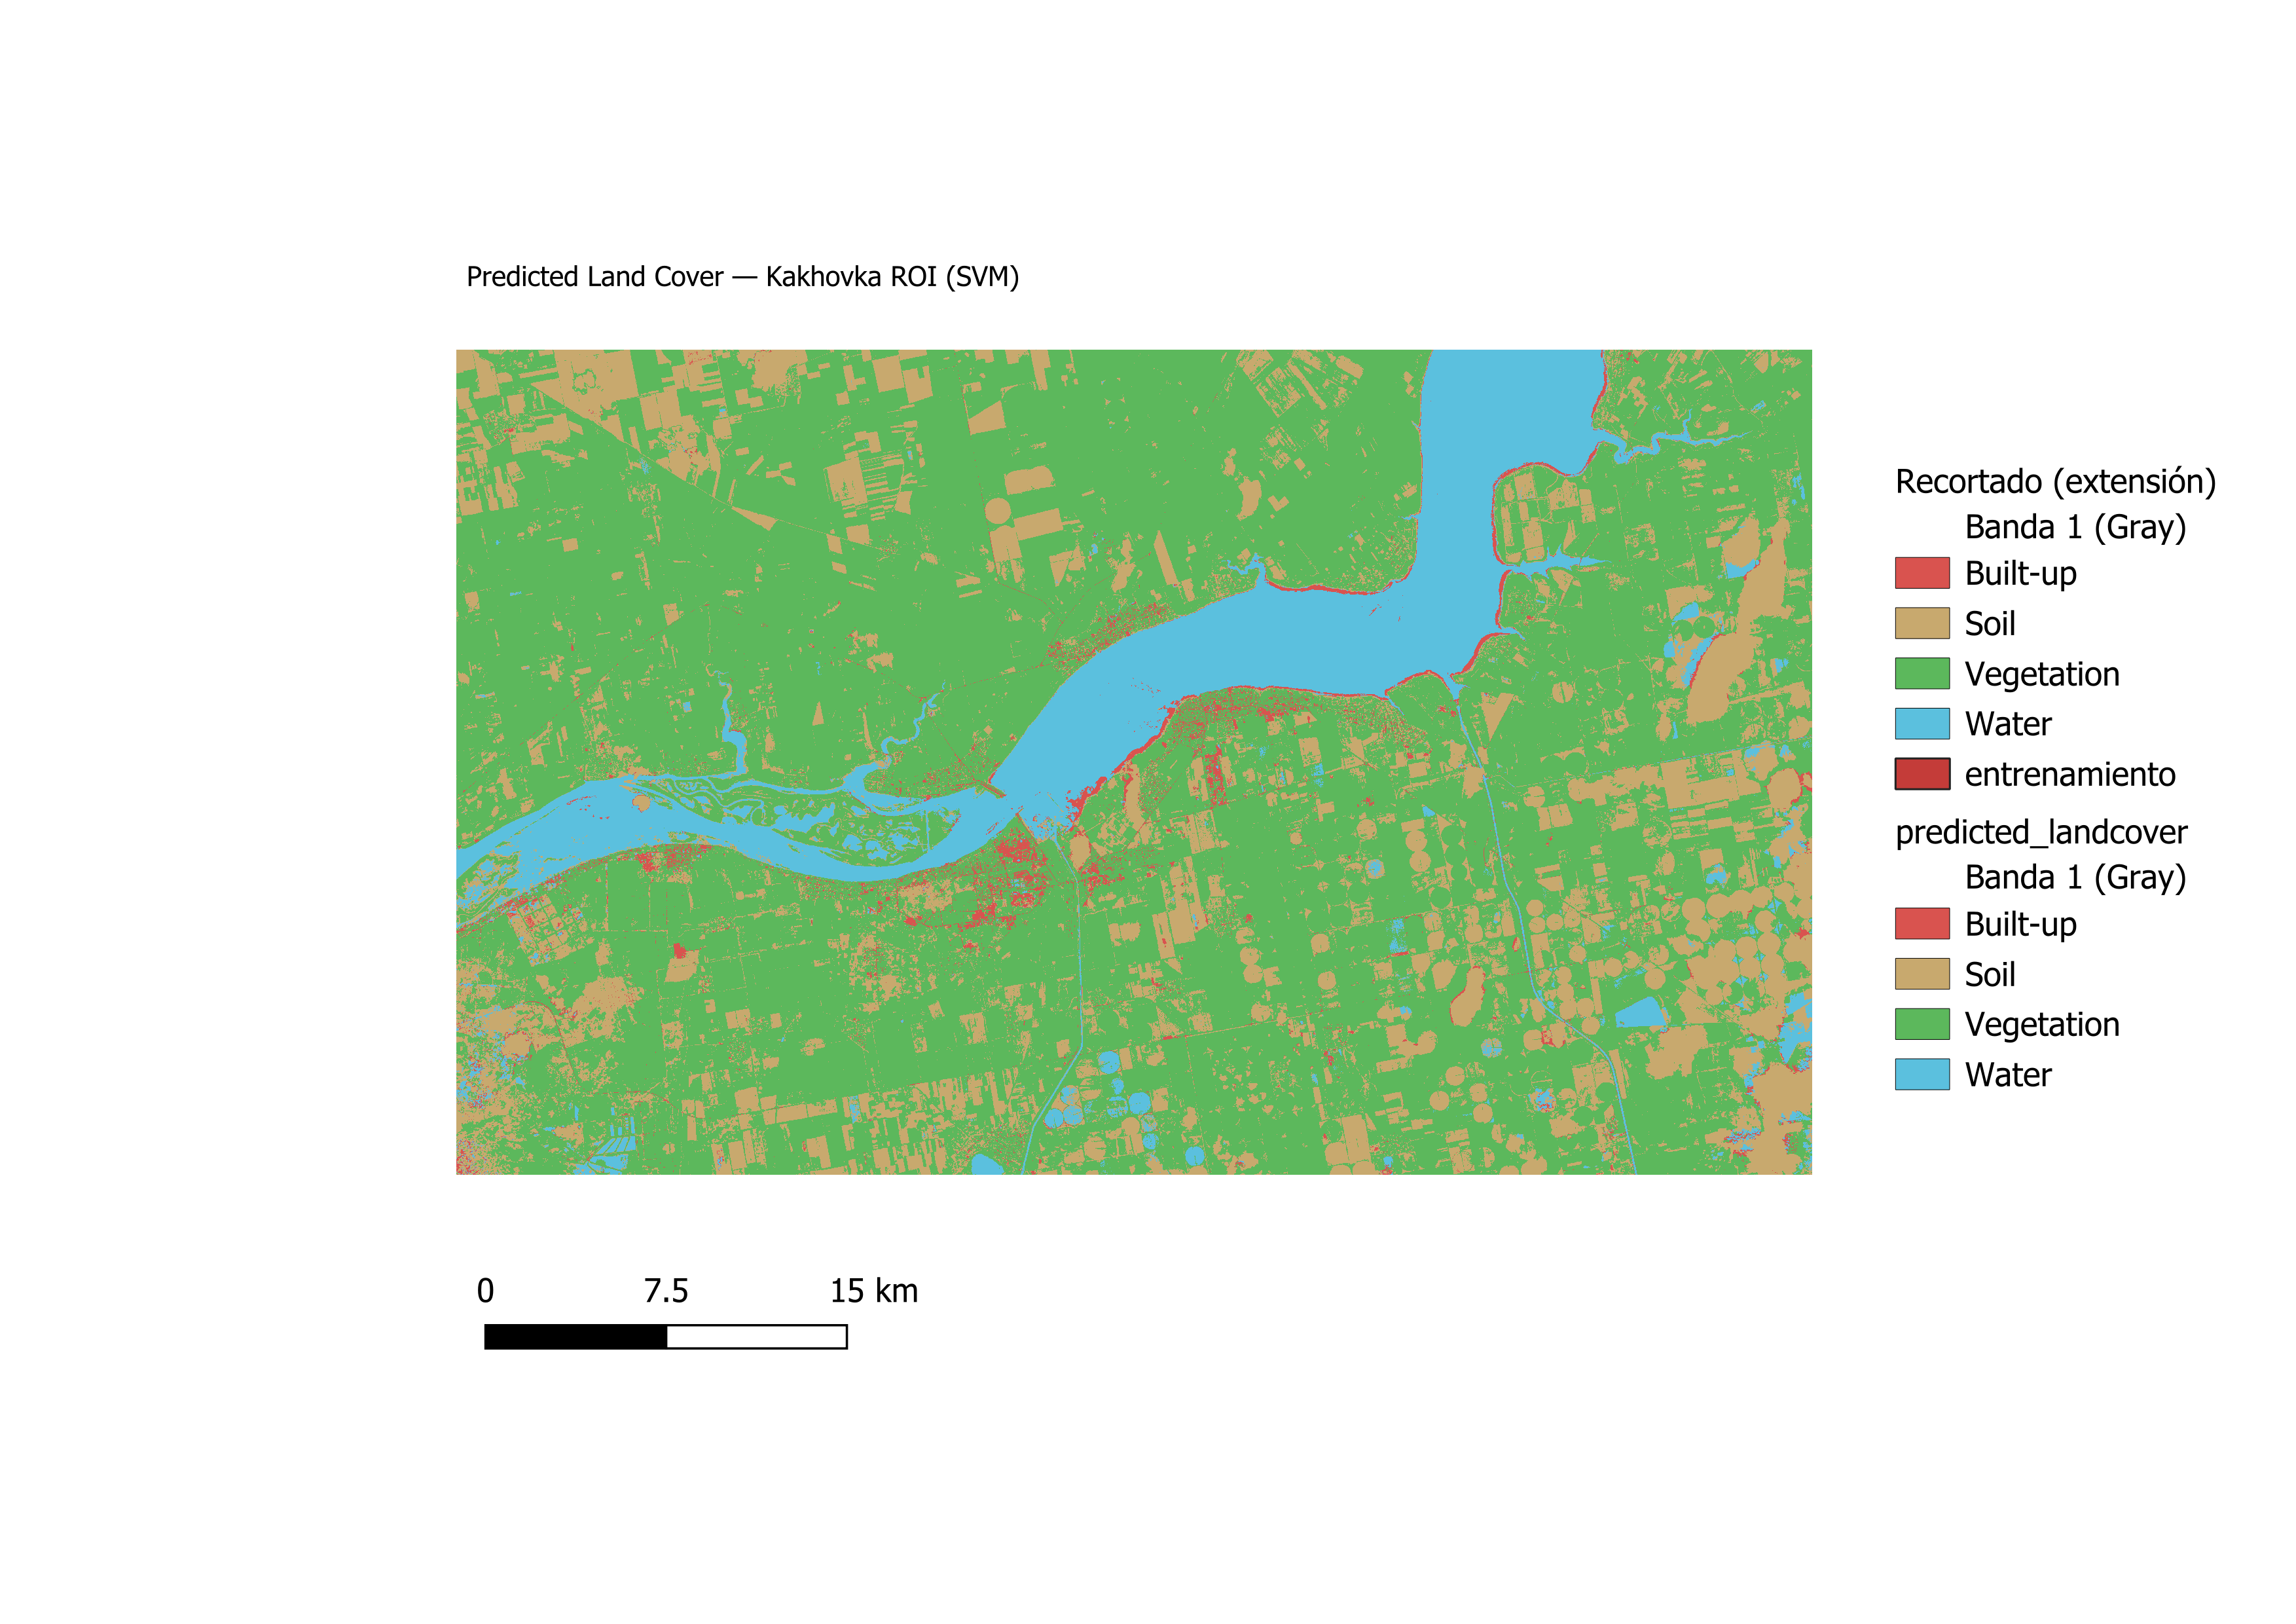
\includegraphics[width=0.95\linewidth]{figures/thematic_map_qgis.png}
    \caption{Predicted land cover map for the Kakhovka post-event Region of
    Interest (SVM classifier, Sentinel-2 post-event image, June 18 2023).
    Classes: Built-up (red), Soil (tan), Vegetation (green), Water (blue).}
    \label{fig:thematic_map}
\end{figure}

Table~\ref{tab:area_per_class} quantifies the total area predicted for each
land cover class within the Region of Interest. Vegetation is the dominant class,
covering 1{,}280.0~km², which reflects the extensive agricultural and riparian
vegetation surrounding the Dnieper River. Soil accounts for 391.8~km², representing
exposed terrain and agricultural bare land following the reservoir drainage. Water
covers 217.7~km², consistent with residual flooding and the river channel in
the post-event scene. Built-up areas represent the smallest fraction at 34.0~km²,
corresponding to the urban footprint of Nova Kakhovka and surrounding settlements.

\begin{table}[H]
\centering
\caption{Estimated area per land cover class derived from the SVM predicted
raster (pixel resolution: 10~m, ROI: $56.2 \times 34.2$~km).}
\label{tab:area_per_class}
\begin{tabular}{lrrr}
\toprule
\textbf{Class} & \textbf{Pixel Count} & \textbf{Area (ha)} & \textbf{Area (km\textsuperscript{2})} \\
\midrule
Built-up   &    339{,}601 &   3{,}396.0 &    34.0 \\
Soil       &  3{,}917{,}935 &  39{,}179.3 &   391.8 \\
Vegetation & 12{,}799{,}655 & 127{,}996.6 & 1{,}280.0 \\
Water      &  2{,}176{,}889 &  21{,}768.9 &   217.7 \\
\midrule
\textbf{Total} & \textbf{19{,}234{,}080} & \textbf{192{,}340.8} & \textbf{1{,}923.4} \\
\bottomrule
\end{tabular}
\end{table}

\end{document}

